\documentclass{article}
\usepackage[T1]{fontenc}
\usepackage[english,brazilian]{babel}
\usepackage{graphicx}
\usepackage[section]{placeins}
\title{Criando um repositório GitHub no Overleaf}
\author{Geraldo Xexéo}
\date{April 2021}

\begin{document}

\maketitle

Uma forma importante de manter um \textit{backup} de tudo que você faz é colocar o Overleaf em controle de versão, no GitHub.

\section{Integrando Overleaf ao GitHub}

É necessário ter uma conta configurada no GitHub para realizar essa integração.

Para integrar sua conta Overleaf com a conta GitHub, do menu principal (lista de projetos) use a opção Account (no canto superior direito) (Figura \ref{fig:accountmenu}) e, na página da sua conta, use o quadro Integração com o GitHub. 

\begin{figure}[hbt]
    \centering
    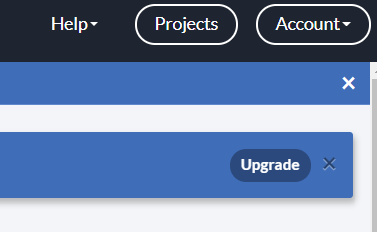
\includegraphics[width=0.9\linewidth]{Image012.png}
    \caption{Menu para chamar a configuração da sua conta.}
    \label{fig:accountmenu}
\end{figure}

Siga então o passo a passo que o Overleaf oferece.

\begin{figure}
    \centering
    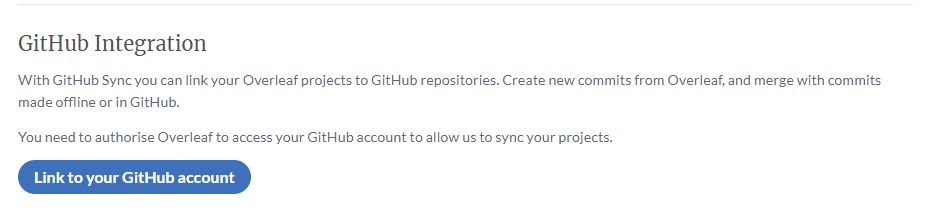
\includegraphics[width=0.6\linewidth]{g1.jpeg}
    \caption{Diálogo de comando para pedir a ligação com o GitHub.}
    \label{fig:g1}
\end{figure}

\begin{figure}
    \centering
    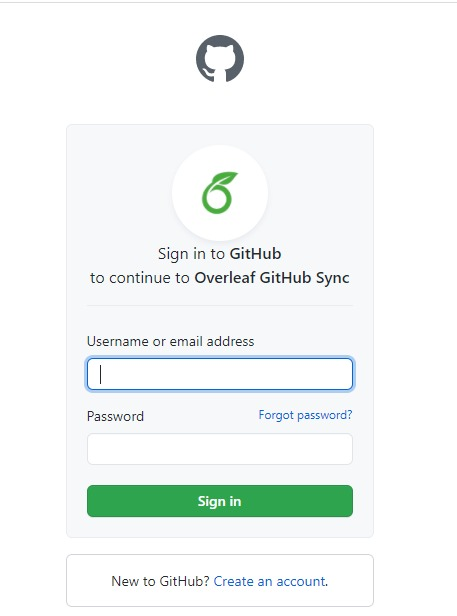
\includegraphics[width=0.6\linewidth]{g11.jpeg}
    \caption{Diálogo para o login do GitHUb}
    \label{fig:g11}
\end{figure}

\begin{figure}
    \centering
    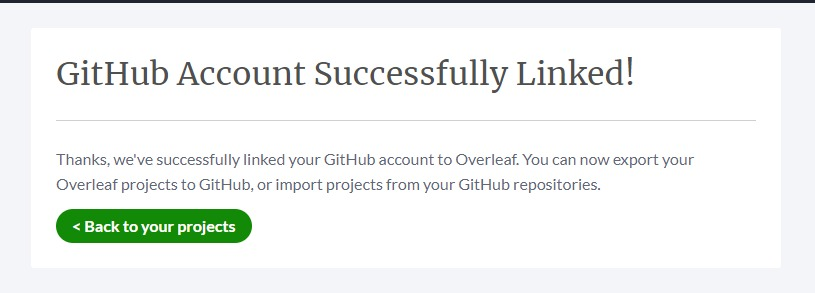
\includegraphics[width=0.9\linewidth]{g2.jpeg}
    \caption{Mensagem de sucesso.}
    \label{fig:g2}
\end{figure}

\begin{figure}
    \centering
    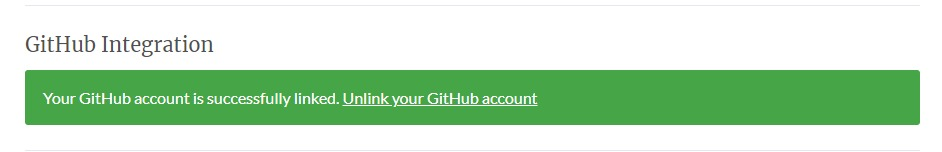
\includegraphics[width=0.9\linewidth]{g3.jpeg}
    \caption{Como fica a configuração da sua conta do Overleaf após o sucesso.}
    \label{fig:g3}
\end{figure}


\section{Criando o repositório}

Para criar o repositório siga os seguintes passos:
\begin{enumerate}
    \item Escolha o Menu no Overleaf;
    \item Escolha a opção GitHub (Figura \ref{fig:git1};
    \item Solicite criar o repositório (Figura \ref{fig:create};
    \item Escolha um nome e lembre de escolher se seu projeto deve se público ou privado (Figura \ref{fig:nomepriv}), ainda podendo escolhar o owner se sua conta contiver organizações;
    \item Dê seu primeiro commit, com push (Figura \ref{fig:commit1}
\end{enumerate}

\begin{figure}[hbt]
    \centering
    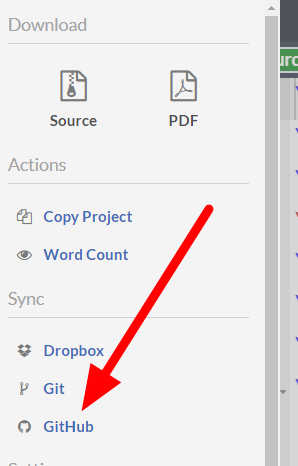
\includegraphics[width=0.5\linewidth]{Image001.png}
    \caption{Escolhendo a opção GitHub}
    \label{fig:git1}
\end{figure}

\begin{figure}[hbt]
    \centering
    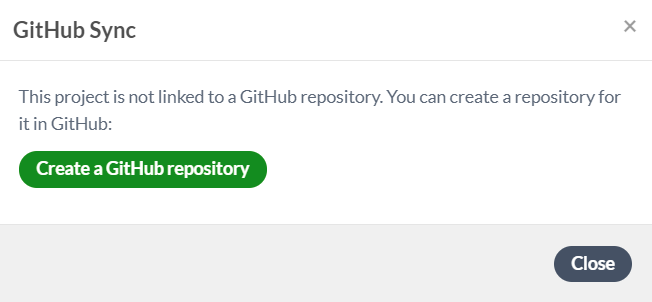
\includegraphics[width=0.9\linewidth]{Image002.png}
    \caption{Mandando criar o repositório}
    \label{fig:create}
\end{figure}

\begin{figure}[hbt]
    \centering
    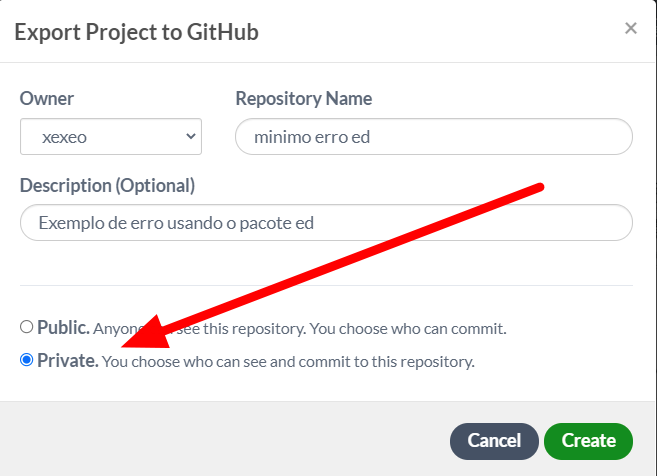
\includegraphics[width=0.9\linewidth]{Image003.png}
    \caption{Escolhendo nome, descrição e opção de privacidade}
    \label{fig:nomepriv}
\end{figure}

\begin{figure}[hbt]
    \centering
    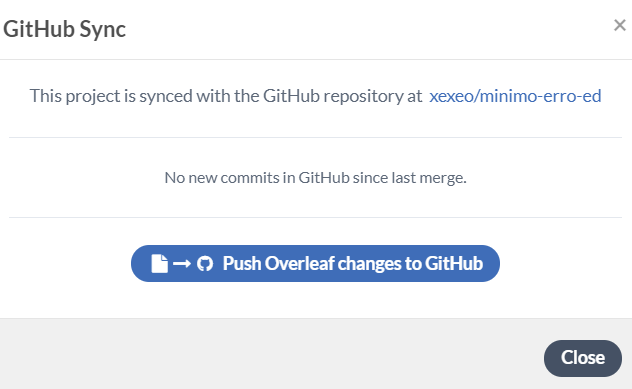
\includegraphics[width=0.9\linewidth]{Image004.png}
    \caption{Primeiro commit e push}
    \label{fig:commit1}
\end{figure}

\section{Atualizando o repositório}

Para atualizar o repositório é necessário usar novamente a opção Menu/GitHub.

A sequência de telas é muito similar a de criação, como mostram as Figuras  \ref{fig:diag1}, \ref{fig:commitpush} e \ref{fig:fimdocp}.

\begin{figure}[hbt]
    \centering
    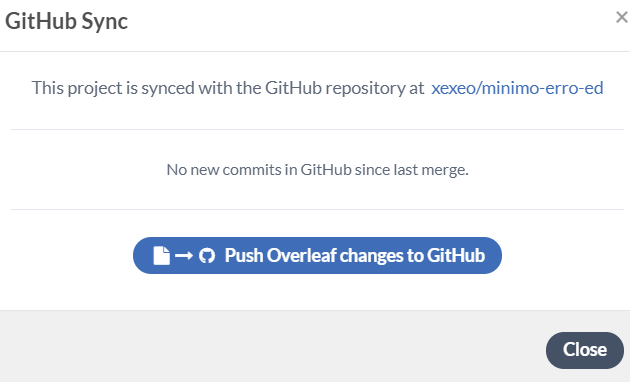
\includegraphics[width=0.9\linewidth]{Image005.png}
    \caption{O diálogo que permite fazer as mudanças}
    \label{fig:diag1}
\end{figure}

\begin{figure}[hbt]
    \centering
    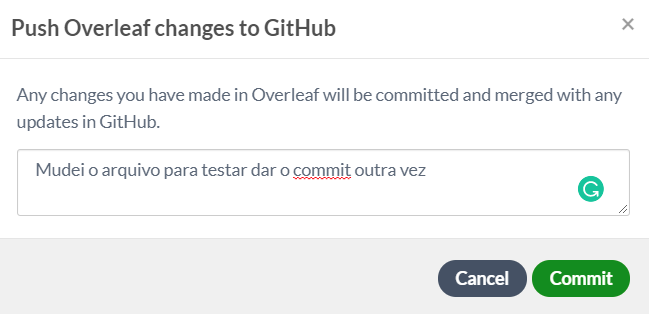
\includegraphics[width=0.9\linewidth]{Image006.png}
    \caption{Identificando o commit-push}
    \label{fig:commitpush}
\end{figure}

\begin{figure}[hbt]
    \centering
    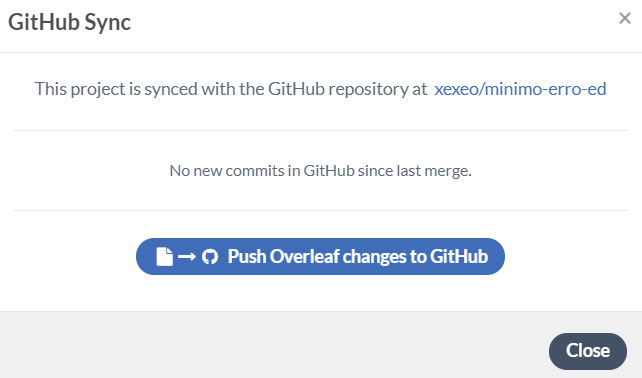
\includegraphics[width=0.9\linewidth]{Image007.png}
    \caption{Fim do commit-push}
    \label{fig:fimdocp}
\end{figure}

\section{Verificando o GitHub}

Se você for ao GitHub, vai encontrar seu repositório novo, como na Figura \ref{fig:repnovo}.

\begin{figure}[hbt]
    \centering
    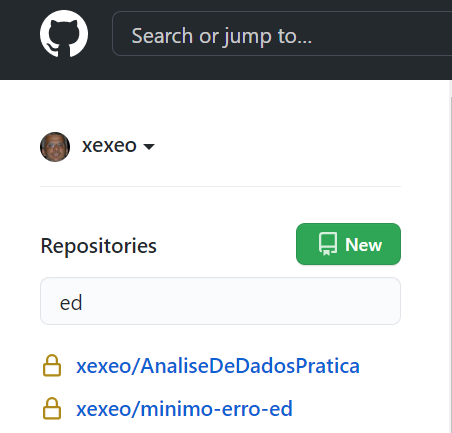
\includegraphics[width=0.6\linewidth]{Image008.png}
    \caption{O repositório novo listado.}
    \label{fig:repnovo}
\end{figure}

Acessando o repositório, você verá os arquivos e a opção Settings (Figura \ref{fig:menurep}), que pode ser usada para adicionar os colaboradores do artigo com suas contas GitHub, onde você deve apertar \textit{Manage Access} e \textit{Invite a Collaborator} (Figura \ref{fig:colinv1}, que levará ao diálogo da Figura \ref{fig:collab}.

\begin{figure}[hbt]
    \centering
    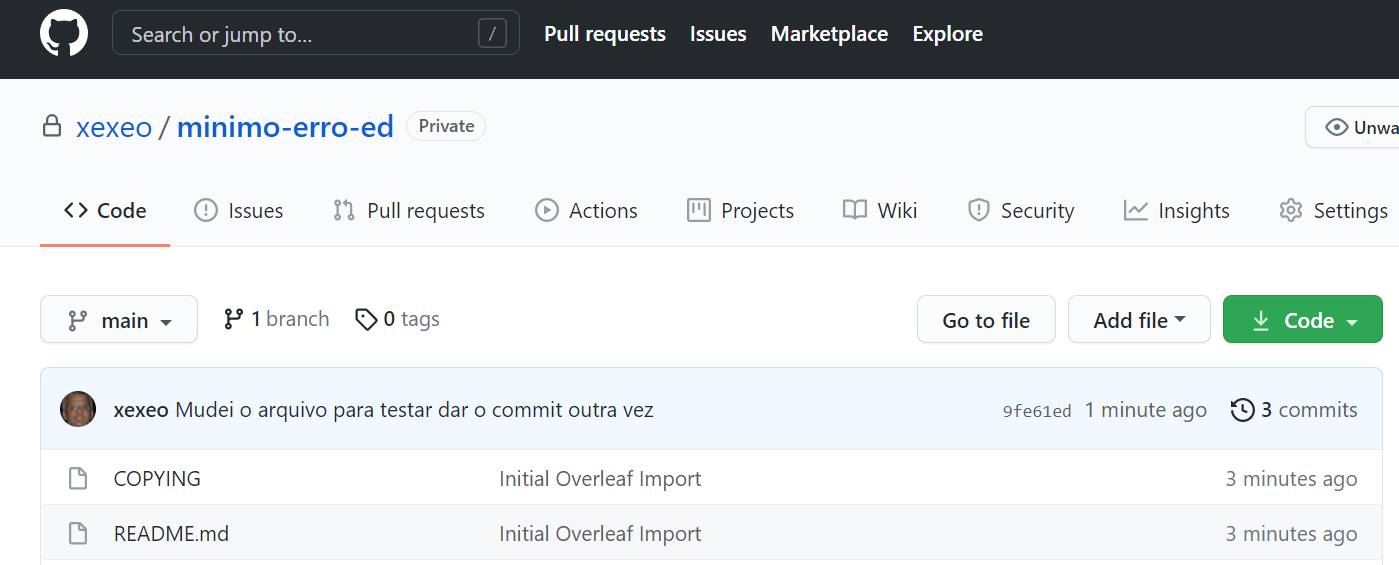
\includegraphics[width=0.9\linewidth]{Image009.png}
    \caption{O menu principal do repositório, com a opção \textit{Settings} ao final.}
    \label{fig:menurep}
\end{figure}

\begin{figure}[hbt]
    \centering
    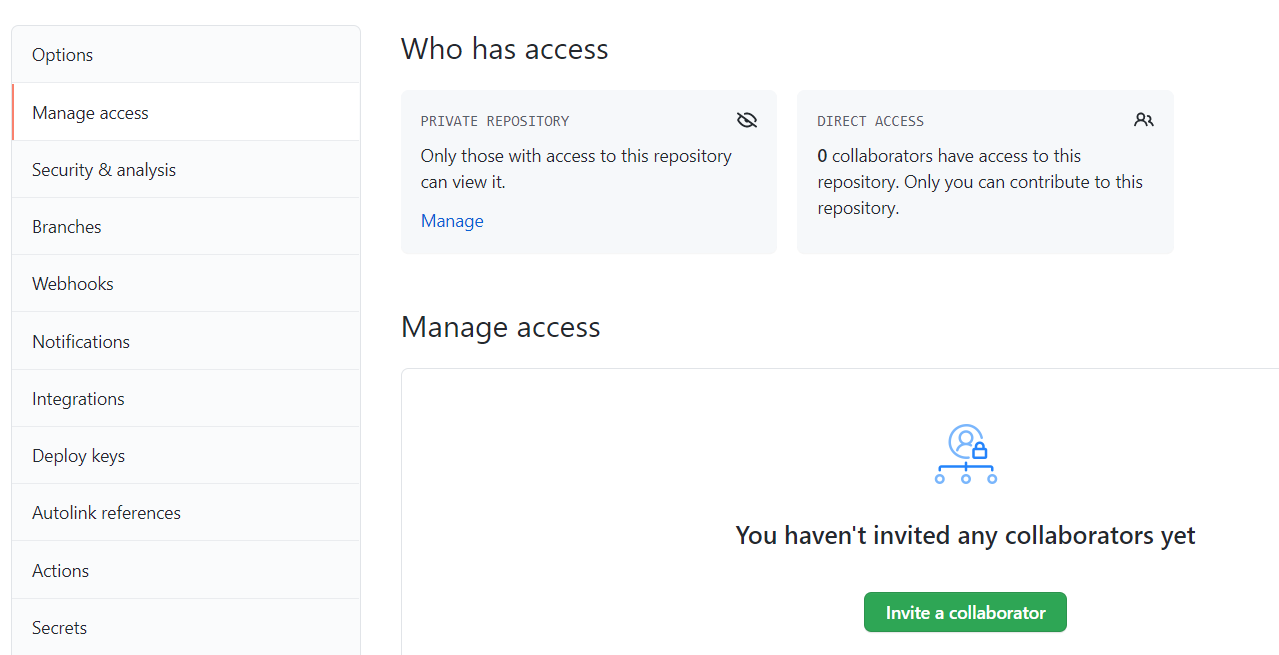
\includegraphics[width=0.9\linewidth]{Image010.png}
    \caption{Para convidar um colaborador, use Manage Access e o botão verde de \textit{Invite a Collaborator}.}
    \label{fig:colinv1}
\end{figure}

\begin{figure}[hbt]
    \centering
    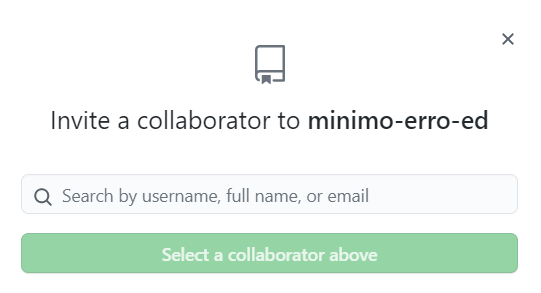
\includegraphics[width=0.9\linewidth]{Image011.png}
    \caption{Diálogo para convidar um colaborador.}
    \label{fig:collab}
\end{figure}

\section{O que acontece se o repositório for alterado por fora?}

A ser feito, mas a princípio siga as instruções do Overleaf.

\section{Um chamado para ajuda}

Se você achar que faltam telas ou explicações nesse arquivo, por favor envie uma mensagem para mim com a informação faltante.

\end{document}
